\begin{blocksection}
\question Write a generator that takes in a tree and yields each possible path from root to leaf, represented as a list of the values in that path.
\newline
For example, consider the tree below. The generator will yield each of the following paths: \lstinline{[1, 2, 5]}, \lstinline{[1, 3, 4]}, \lstinline{[1, 3, 6]}, and \lstinline{[1, 7]}.
\newline
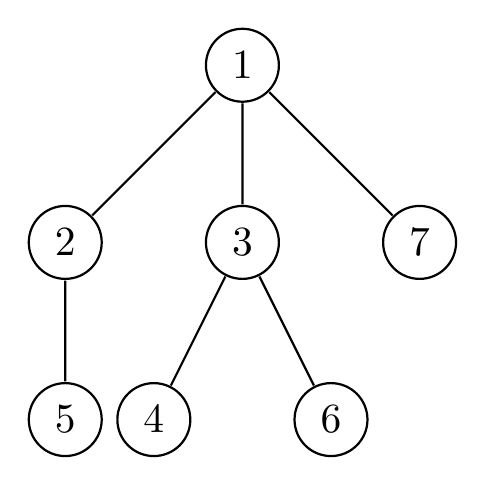
\begin{tikzpicture}[thick, scale=1.5, transform shape]
    \node [circle, draw] (z){$1$}
        child {node [circle, draw] (a) {$2$}
            child {node [circle, draw] (d) {$5$}}
        }
        child {node [circle, draw] (b) {$3$}
            child {node [circle, draw] (e) {$4$}}
            child {node [circle, draw] (f) {$6$}}
        }
        child {node [circle, draw] (c) {$7$}};
\end{tikzpicture}
\newline
\begin{lstlisting}
def all_paths(t):
    """
    >>> t = Tree(1, [Tree(2, [Tree(5)]), Tree(3, [Tree(4), Tree(6)]), Tree(7)])
    >>> print(list(all_paths(t)))
        [[1, 2, 5], [1, 3, 4], [1, 3, 6], [1, 7]]
    """    
    if _________________________:

        _________________________

    else:

        for _____________________________:

            for _____________________________:

                ______________________________
\end{lstlisting}
\end{blocksection}
\begin{blocksection}
\begin{solution}[0in]
\begin{lstlisting}
    if t.is_leaf():
        yield [t.label]
    for b in t.branches:
        for subpath in all_paths(b):
            yield [t.label] + subpath
\end{lstlisting}

\end{solution}
\end{blocksection}
